\subsection*{Cross-Site Request Forgery -- Profile Update (CSRF)}

\begin{table}[H]
\centering
\begin{tabular}{|l|p{10cm}|}
\hline
\textbf{Finding ID} & CSRF \\
\hline
\textbf{Severity} & Medium \\
\hline
\textbf{CVSS 3.1 Score} & 4.3 (Medium) \\
\hline
\textbf{CVSS Vector} & \texttt{AV:N/AC:L/PR:N/UI:R/S:U/C:N/I:L/A:N} \\
\hline
\textbf{Status} & Confirmed \\
\hline
\textbf{OWASP Category} & A01:2021 -- Broken Access Control \\
\hline
\textbf{CWE} & CWE-352 -- Cross-Site Request Forgery (CSRF) \\
\hline
\textbf{Affected Endpoint} & \texttt{POST /profile} \\
\hline
\textbf{Affected Parameter} & \texttt{username} \\
\hline
\end{tabular}
\caption{CSRF finding details}
\end{table}

\subsubsection*{Description}

The profile update functionality does not provide sufficient
protection against Cross-Site Request Forgery (CSRF) attacks.

The profile update request does not contain a CSRF protection token.
A malicious external HTML page can therefore create and automatically
submit a request to the \texttt{/profile} endpoint while the victim
is authenticated.

During testing, the username of the authenticated user was changed
to an attacker-controlled value by opening the malicious HTML page.

\subsubsection*{Methodology}

The vulnerability was identified by intercepting the profile update
request using Burp Suite.

The request was reviewed to determine whether a CSRF token or other
effective CSRF protection mechanism was present.

A proof-of-concept HTML page was then created containing a form that
submitted a POST request to the profile endpoint. The form was
automatically submitted using JavaScript.

The test was performed while a user was authenticated to the
application. The username was successfully changed to the value
specified in the malicious form, confirming the CSRF vulnerability.

\subsubsection*{Steps to Reproduce}

\begin{enumerate}

    \item Log in to the OWASP Juice Shop application using a valid
    user account.

    \item Open the profile page and intercept the username update
    request using Burp Suite.

    \item Observe that the profile update request does not contain a
    CSRF protection token.

    \item Create a malicious HTML file containing the following form:

    \begin{lstlisting}
<form action="http://127.0.0.1:3000/profile" method="POST">
    <input name="username" value="CSRF"/>
</form>
<script>document.forms[0].submit();</script>
    \end{lstlisting}

    \item Save the file as \texttt{csrfjuice.html}.

    \item While still authenticated to the Juice Shop application,
    open the malicious HTML file.

    \item Observe that the form is automatically submitted to the
    \texttt{/profile} endpoint.

    \item Return to the Juice Shop profile and observe that the
    username has been changed to the attacker-controlled value.

\end{enumerate}

\subsubsection*{Evidence}

The following evidence demonstrates the missing CSRF protection,
the proof-of-concept payload, and the successful execution of the
attack.

\begin{figure}[H]
    \centering
    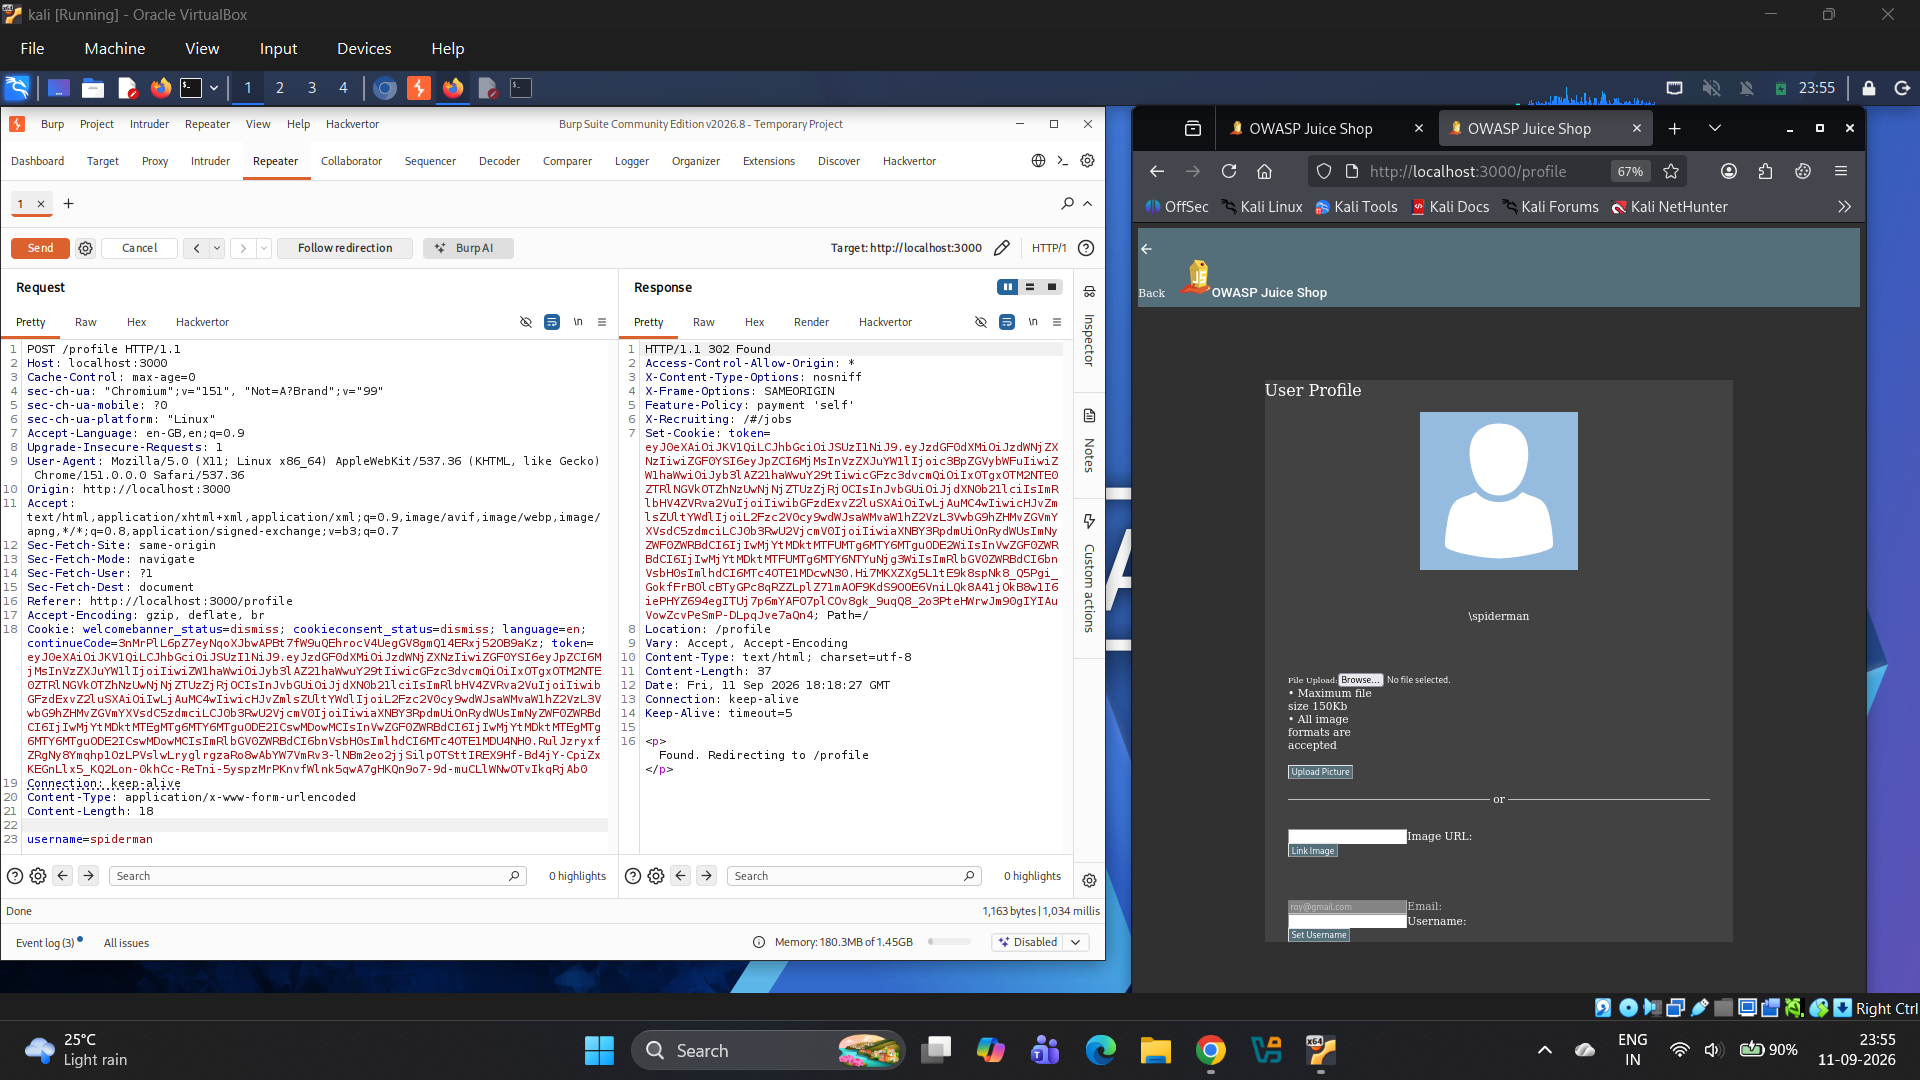
\includegraphics[width=0.8\textwidth]{
        evidence/phase4/csrf/01_burp_profile_post_no_token.png
    }
    \caption{Burp Suite showing the profile update request without a CSRF token}
    \label{fig:csrf-burp-request}
\end{figure}

\begin{figure}[H]
    \centering
    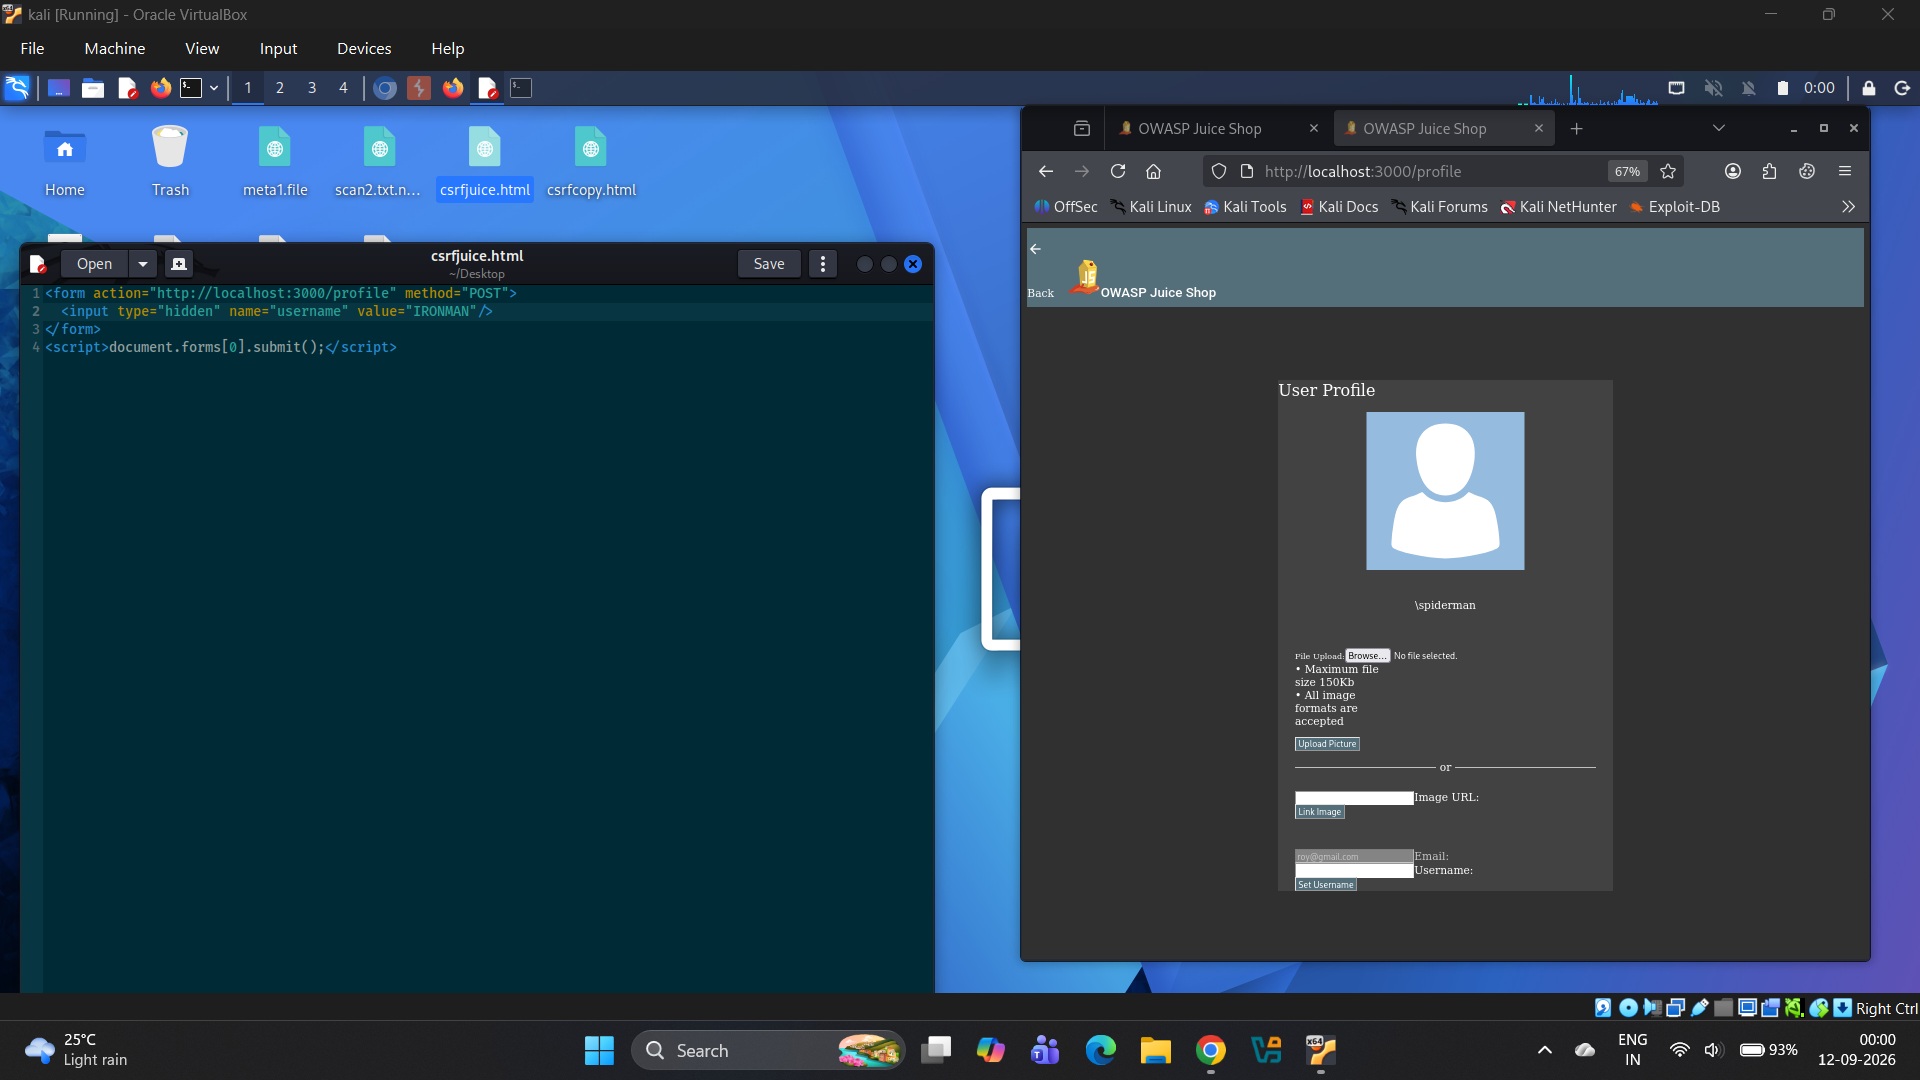
\includegraphics[width=0.8\textwidth]{
        evidence/phase4/csrf/02_csrf_payload_source.png
    }
    \caption{CSRF proof-of-concept HTML form used to submit the request automatically}
    \label{fig:csrf-payload}
\end{figure}

\begin{figure}[H]
    \centering
    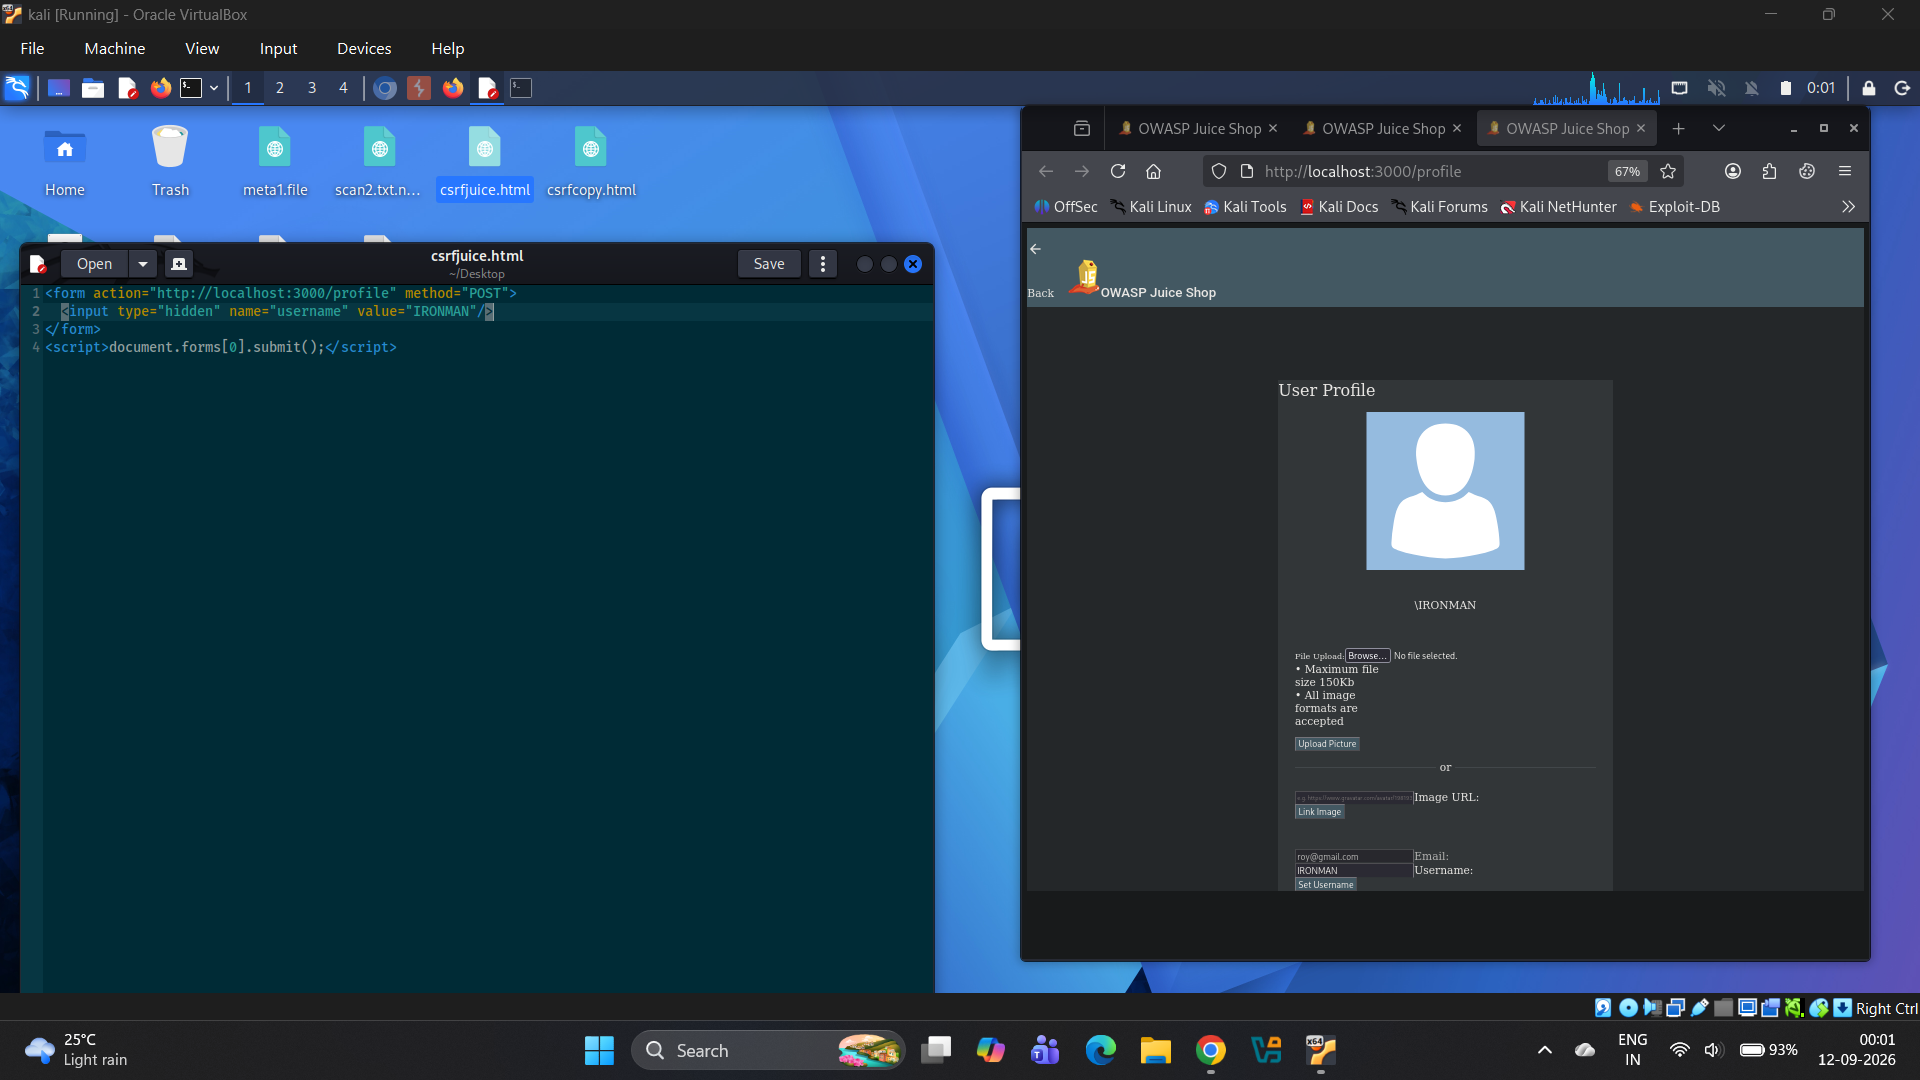
\includegraphics[width=0.8\textwidth]{
        evidence/phase4/csrf/03_username_changed_result.png
    }
    \caption{Successful username change after the CSRF payload was executed}
    \label{fig:csrf-success}
\end{figure}

\subsubsection*{Impact}

An attacker can create a malicious webpage that submits an unwanted
profile update request when an authenticated victim visits the page.

In this case, the attacker can change the victim's username without
requiring the victim to manually submit the profile update form.

If similar CSRF protection is missing from other sensitive operations,
the impact could be greater depending on the actions available to an
authenticated user.

\subsubsection*{Remediation}

\begin{itemize}

    \item Implement a strong, unpredictable CSRF token for
    state-changing requests.

    \item Validate the CSRF token on the server side before processing
    the request.

    \item Use appropriate SameSite cookie settings as an additional
    layer of protection.

    \item Apply CSRF protection consistently to all sensitive
    state-changing operations.

    \item Do not rely only on client-side validation for CSRF
    protection.

\end{itemize}

\subsubsection*{Conclusion}

The CSRF vulnerability was successfully confirmed through manual
testing. A malicious HTML page was able to submit a profile update
request while the victim was authenticated, resulting in an
attacker-controlled username change.

The finding is therefore classified as a confirmed Medium-severity
security issue.



